\chapter{GSM}

\section{Overview}

GSM (Global System for Mobile Communications, originally Groupe Sp\'ecial Mobile), is a very popular standard that describes protocols for second generation (2G) digital cellular networks used by mobile phones. GSM networks usually operate in the 900 MHz, 1800 MHz or 1900 MHz bands. It supports a full data rate of 9.6 kbits/sec or 14.4 kbits/sec using better codecs.


\subsection{System Architecture}

A GSM Public Land Mobile Network (PLMN) consists of at least one Service Area managed by a Mobile Switching Center (MSC) connected to the Public Switched Telephone Network  (PSTN).

\begin{figure}
\centering
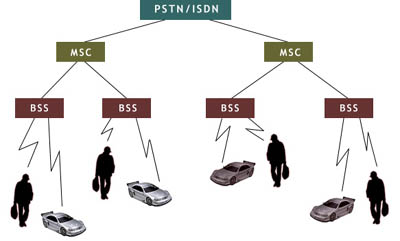
\includegraphics[scale=0.7]{archPLMN}
\caption[GSM PLMN architecture]{The architecture of a GSM Public Land Mobile Network (PLMN).
\emph{Source: \url{http://wireless.arcada.fi/MOBWI/material/CN\_1\_2.html}}}
\end{figure}

The network structure can be divided into the following discrete sections:
\begin{itemize}
\item Base Station Subsystem
\item Network and Switching Subsystem
\item Operation Subsystem
\end{itemize}


\subsubsection{Base Station Subsystem (BSS)}

A base station subsystem consists of
\begin{itemize} 
\item a Base Station Controller (BSC) and
\item at least one Base Transceiver Station (BTS) for Mobile Stations (MS). A mobile station can be a cell phone, or any electronic equipment such as a Personal Digital Assistant (PDA) with a phone interface.
\end{itemize}

The area served by a single BTS is considered a Network Cell. One or more BTSs are managed by a single BSC.  A group of BSSs can be managed as a Location Area (Location Area) if all those BSSs are being managed by the same MSC.


\begin{figure}
\centering
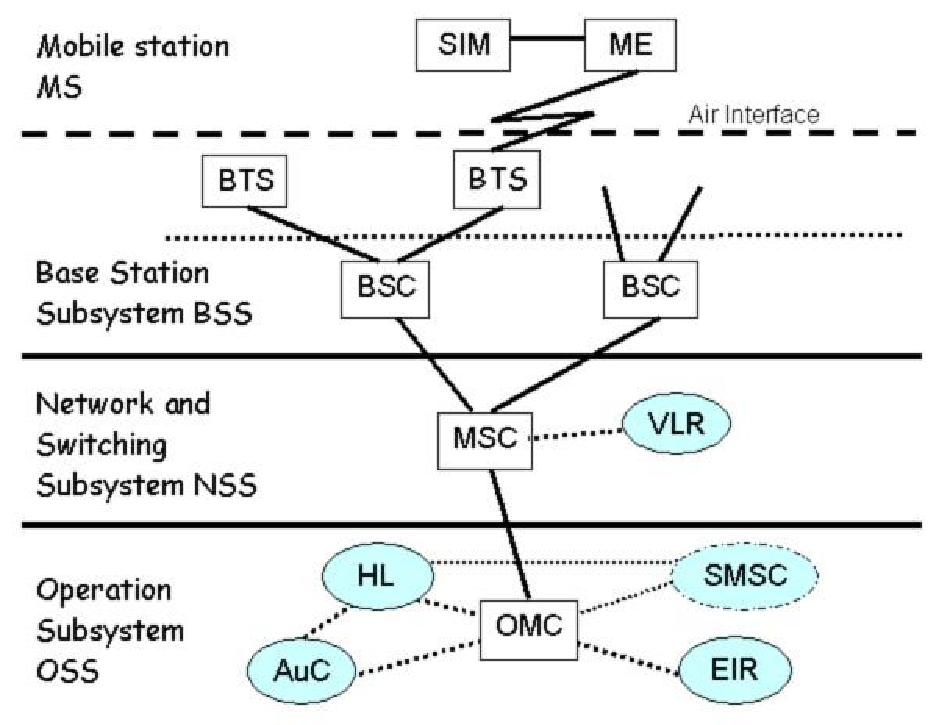
\includegraphics[scale=0.7]{archMSCServiceArea}
\caption[Network architecture for a single MSC Service Area]{The GSM network architecture for a single MSC controlled Service Area.
\emph{Source: \url{http://wireless.arcada.fi/MOBWI/material/CN\_1\_2.html}}}
\end{figure}


An MSC may also be connected via a Gateway MSC (GMSC) to other MSCs or the Public Switched Telephone Network (PSTN) with the Integrated Services Digital Network (ISDN) option. The Inter-Working Function (IWF) of a GMSC makes it possible to connect the circuit switched data paths of a GSM network with the PSTN/ISDN.

\begin{figure}
\centering
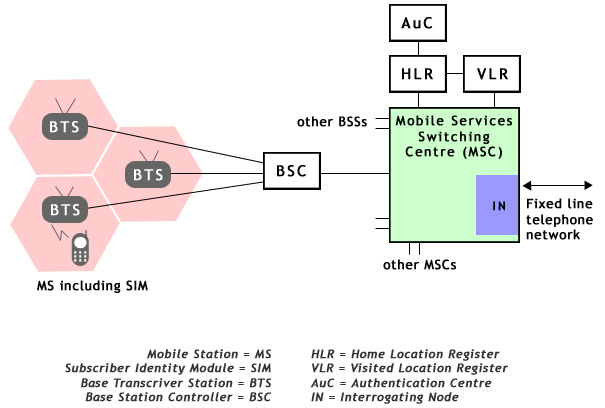
\includegraphics[scale=0.7]{gsmNetworkComponents}
\caption[GSM network components]{GSM network components.
\emph{Source: \url{http://wireless.arcada.fi/MOBWI/material/CN\_1\_2.html}}}
\end{figure}




\subsubsection{Network and Switching Subsystem (NSS)}

The NSS is made up of an MSC and a Visitor Location Register (VLR). An MSC 
\begin{itemize} 
\item sets up, controls and shuts down connections
\item handles call charges
\item manages additionals services like call forwarding, call blocking, etc.
\end{itemize}

A VLR contains all the subscriber data of the phones being served by the accompanying MSC. It contains their location data too. The VLR also maintains data about the SIMs that do not belong to the network but have roamed into the network. The area served by an MSC is called a MSC/VLR service area.

\begin{figure}
\centering
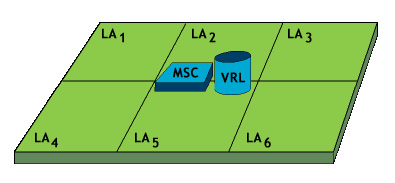
\includegraphics[scale=0.7]{mscvlrServiceArea}
\caption[MSC/VLR Service Area]{MSC/VLR Service Area.
\emph{Source: \url{http://wireless.arcada.fi/MOBWI/material/CN\_1\_2.html}}}
\end{figure}

\subsubsection{The Operation Subsystem (OSS)}

The OSS consists of :
\begin{itemize}
\item the Operation and Maintenance Center (OMC)
\item the Authentication Center (AuC)
\item the Home Location Register (HLR)
\item the Equipment Identity Register (EIR)
\end{itemize}

The OSS is responsible for
\begin{itemize}
\item network management functions like service provisioning, network configuration, fault management, etc.
\item billing calls
\item administering subscribers
\end{itemize}

The AuC controls all the encryption algorithms used for verifying the SIMs. The EIR contains the serial numbers of all the MSs (mobile phones) being served. The HLR contains the subscriber data and location data of all the SIMs in different parts of the network.

\subsubsection{GSM Network Areas}

The area covered by a GSM operator is called a PLMN Service Area. A PLMN service area is made up of several MSC/VLR service areas. The hierarchy of service areas is as follows:
\begin{itemize}
\item PLMN service area,
\item MSC/VLR service area,
\item Location Area and
\item Network Cell
\end{itemize}
\begin{figure}
\centering
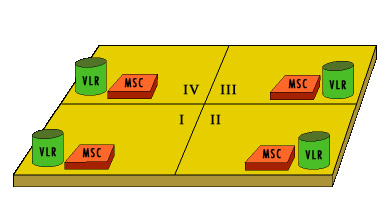
\includegraphics[scale=0.7]{PLMNServiceArea}
\caption[A PLMN Service Area for a GSM operator]{A PLMN Service Area for a GSM operator.
\emph{Source: \url{http://wireless.arcada.fi/MOBWI/material/CN\_1\_2.html}}}
\end{figure}

